% !TeX TS-program = latexmk % | dvisvgm --pdf --exact --font-format=woff --zoom=-1 %.pdf | txs:///view-log | txs:///view-pdf 
\documentclass{standalone}
\usepackage{tikzducks}

\newcommand{\towelpath}{%
	(1.1676,0.3641) .. controls (1.1676,0.3641) and (1.3763,0.4825) .. (1.4605,0.4542) .. controls (1.5447,0.4259) and (1.4874,0.2742) .. (1.5769,0.2627) .. controls (1.6664,0.2513) and (1.7126,0.4470) .. (1.8022,0.4655) .. controls (1.8918,0.4839) and (1.9360,0.3787) .. (2.0087,0.4054) .. controls (2.0814,0.4321) and (2.0834,0.4936) .. (2.1476,0.5744) .. controls (2.1292,0.6964) and (1.9783,1.1341) .. (1.8735,1.2390) .. controls (1.6974,1.2913) and (1.2567,1.2394) .. (1.2089,1.1676) .. controls (1.1418,1.0668) and (1.1676,0.3641) .. (1.1676,0.3641) -- cycle;
}

\pagecolor{gray!20!white}

\begin{document}
	
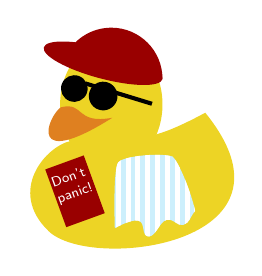
\begin{tikzpicture}[scale=1.3]
% duck %%%%%%%%%%%%%%%%%%%%%%%%%%%%%%%%%%%%%%%%%%%%%%%%%%%%%%%%%%%%%%
	\duck[%
		cap=red!60!black,
		sunglasses,
%		signpost={\Large \sffamily \color{black} Rio?},
%		signcolour=gray,
%		signback=brown!20!white,
	]
% towel %%%%%%%%%%%%%%%%%%%%%%%%%%%%%%%%%%%%%%%%%%%%%%%%%%%%%%%%%%%%%%
	\begin{scope}[scale=0.8]
		\fill[cyan!20!white] \towelpath;
		\begin{scope}
			\clip \towelpath;
			\foreach \shifta in {0,0.12,...,2.4}{%
				\fill[white,rotate around={0:(1.2,0.9)}] 
				($(0.1,-0.3)+(\shifta,0)$) rectangle ($(0.1,-0.3)+(\shifta,0)+(0.06,2.7)$);
			}
		\end{scope}
	\end{scope}
% book %%%%%%%%%%%%%%%%%%%%%%%%%%%%%%%%%%%%%%%%%%%%%%%%%%%%%%%%%%%%%%%
	\begin{scope}[rotate=40,yshift=-14,xshift=-1]
		\fill[red!60!black,rotate=-20] (0.40,1.20) rectangle (0.80,0.60);
		\node[rotate=20, color=white] at (0.88,0.70) {\parbox{0.45cm}{\tiny \sffamily Don't panic!}};
	\end{scope}
\end{tikzpicture}	
	
\end{document}